\section{\crossflow Architecture and Design}
\label{sec:architecture}

In this section, we motivate and describe the architecture and design of \crossflow. In Section~\ref{sec:data_plane}, we introduce the proposed data plane abstractions. Then, in Section~\ref{sec:messages}, we describe how we extend the OpenFlow protocol to accommodate \crossflow messages.

%\begin{figure}[t]
%  \centering
%  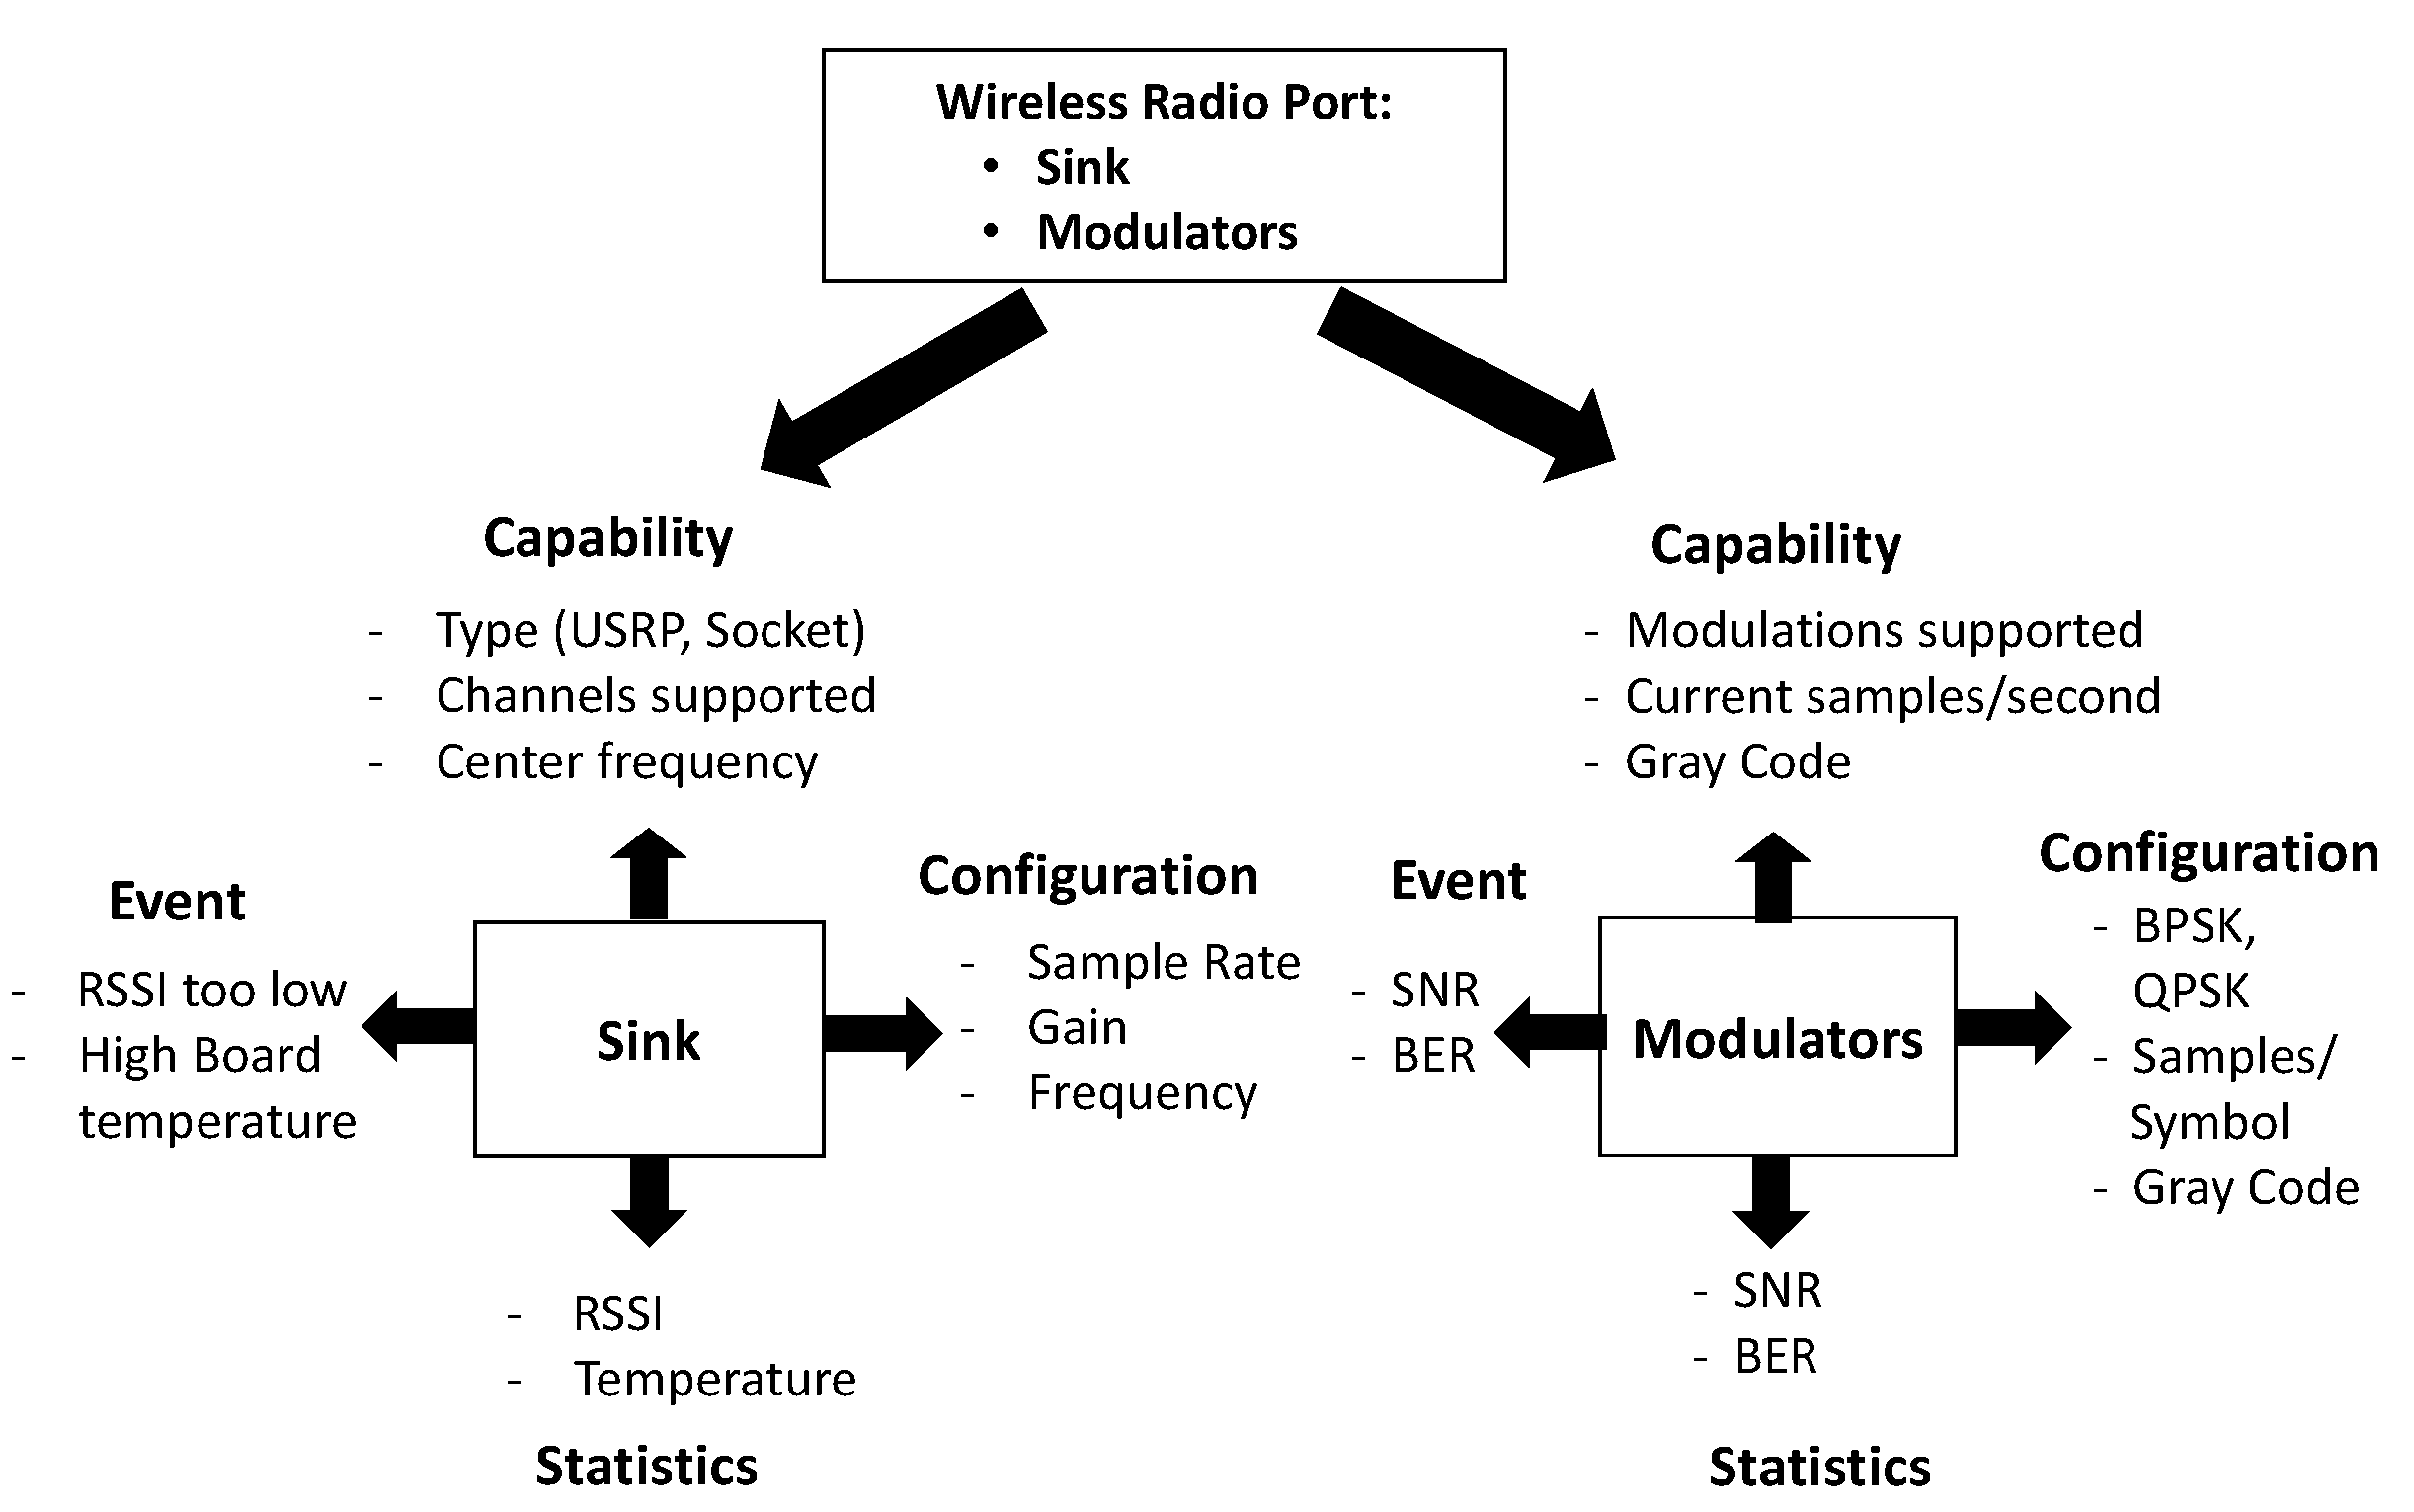
\includegraphics[width=0.48\textwidth]{figures/Interfaces.pdf}
%  \caption{Interface model for wireless radio port abstraction with two processing blocks: Sink and Modulators}
%  \label{fig:interface}
%\end{figure}

\begin{figure}[t]
  \centering
  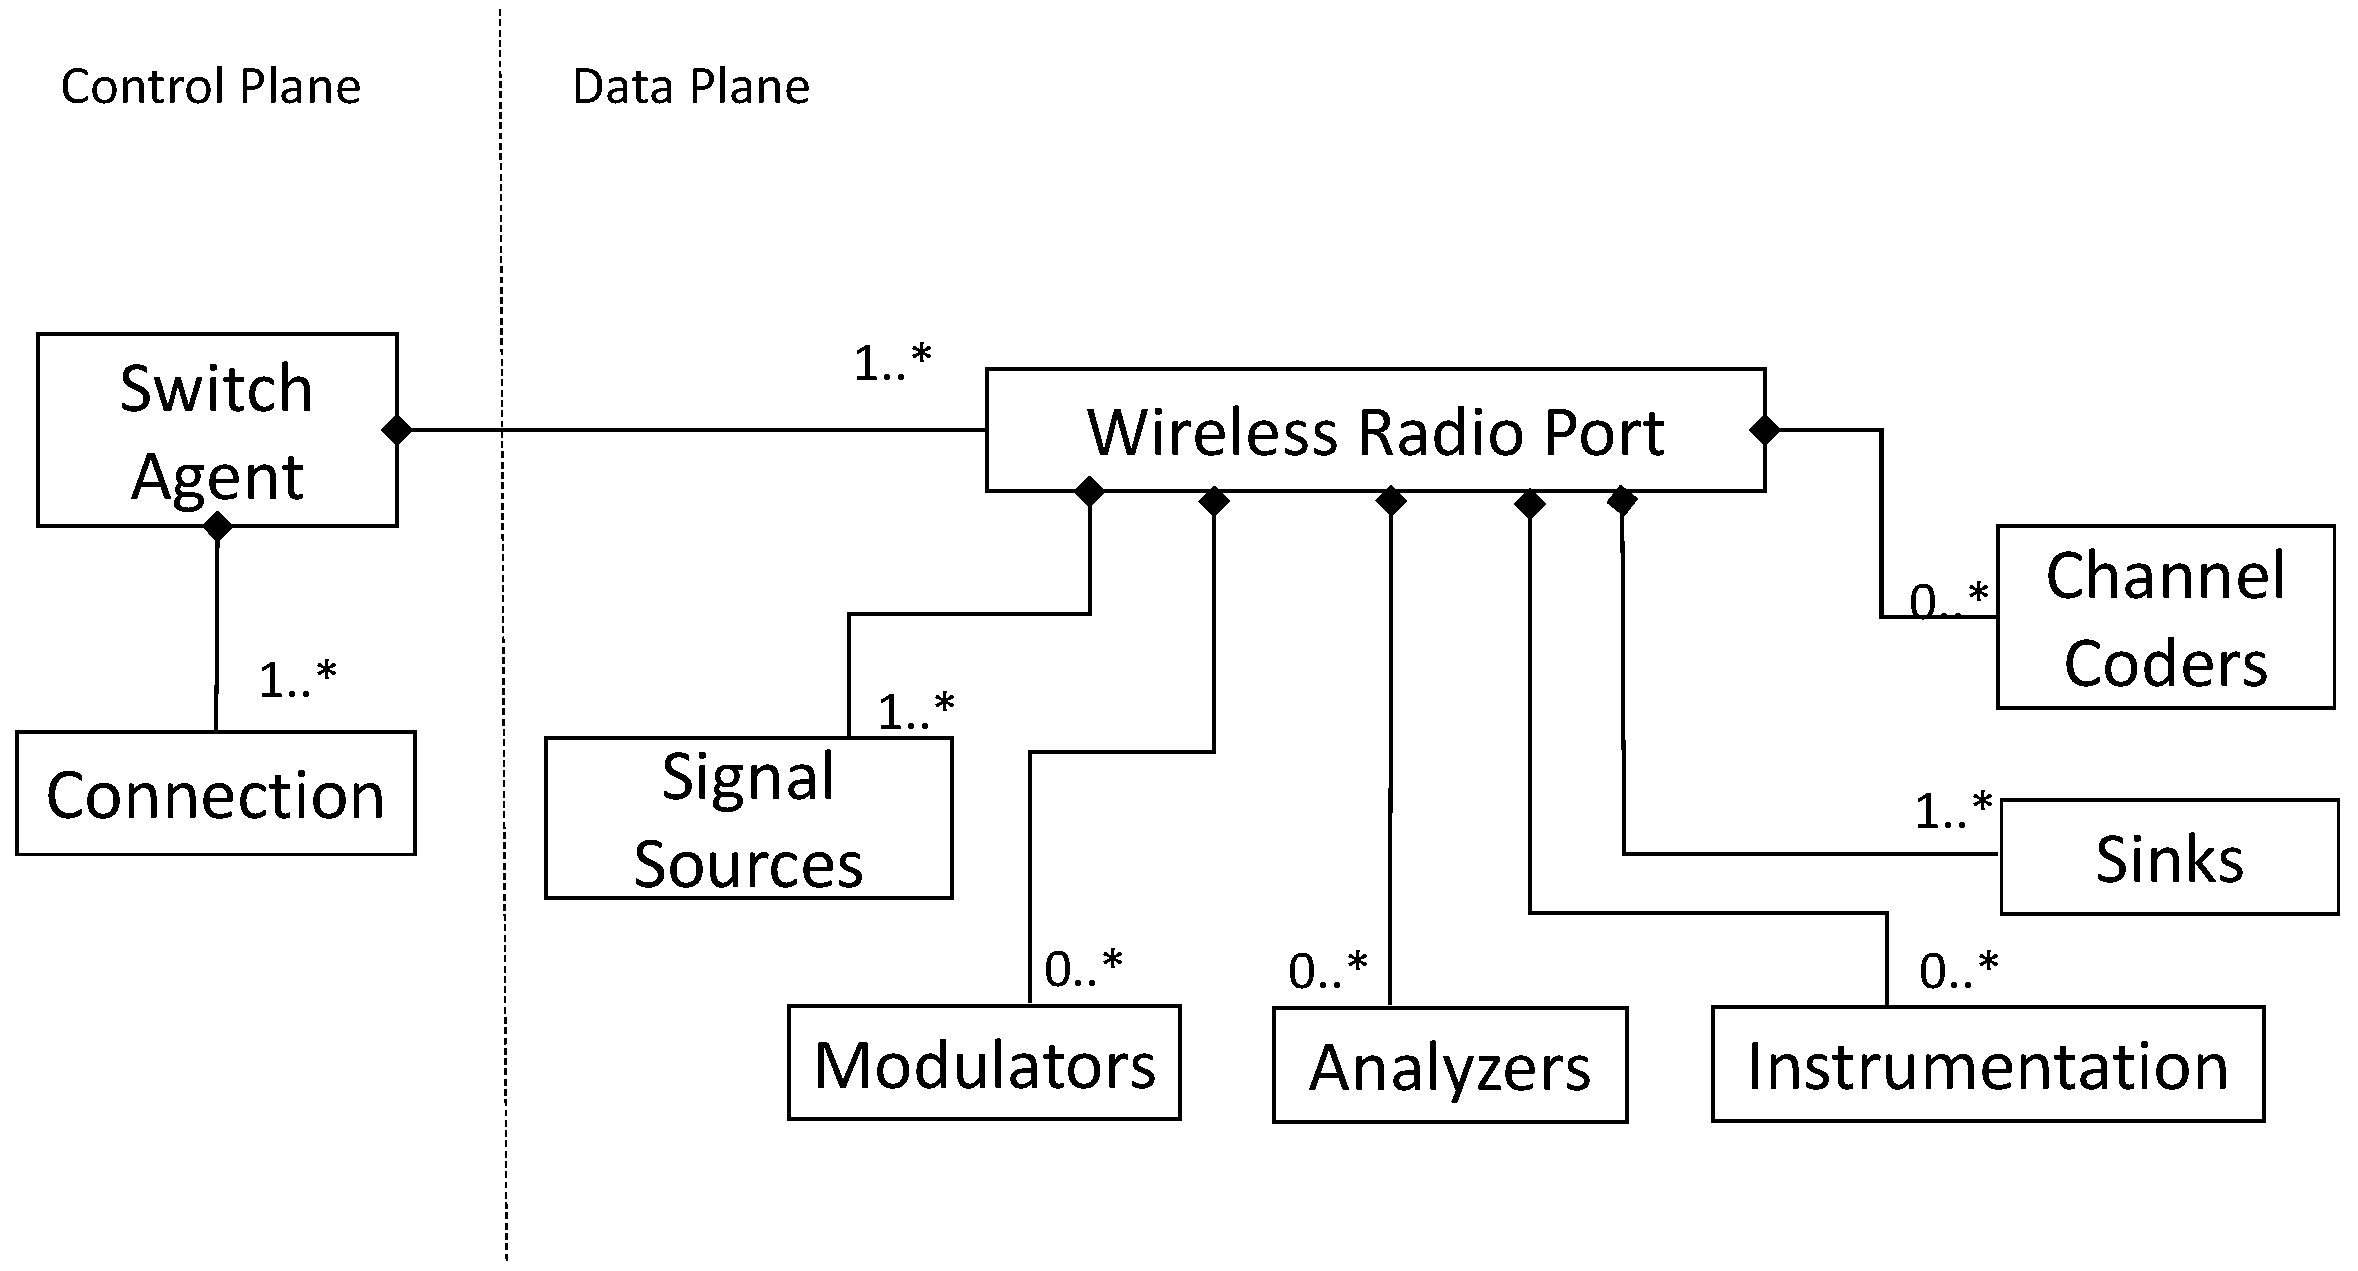
\includegraphics[width=0.48\textwidth]{figures/UML.pdf}
  \caption{Abstraction model of \crossflow}
  \label{fig:uml}
\end{figure}

%\begin{figure*}
%  \centering
%  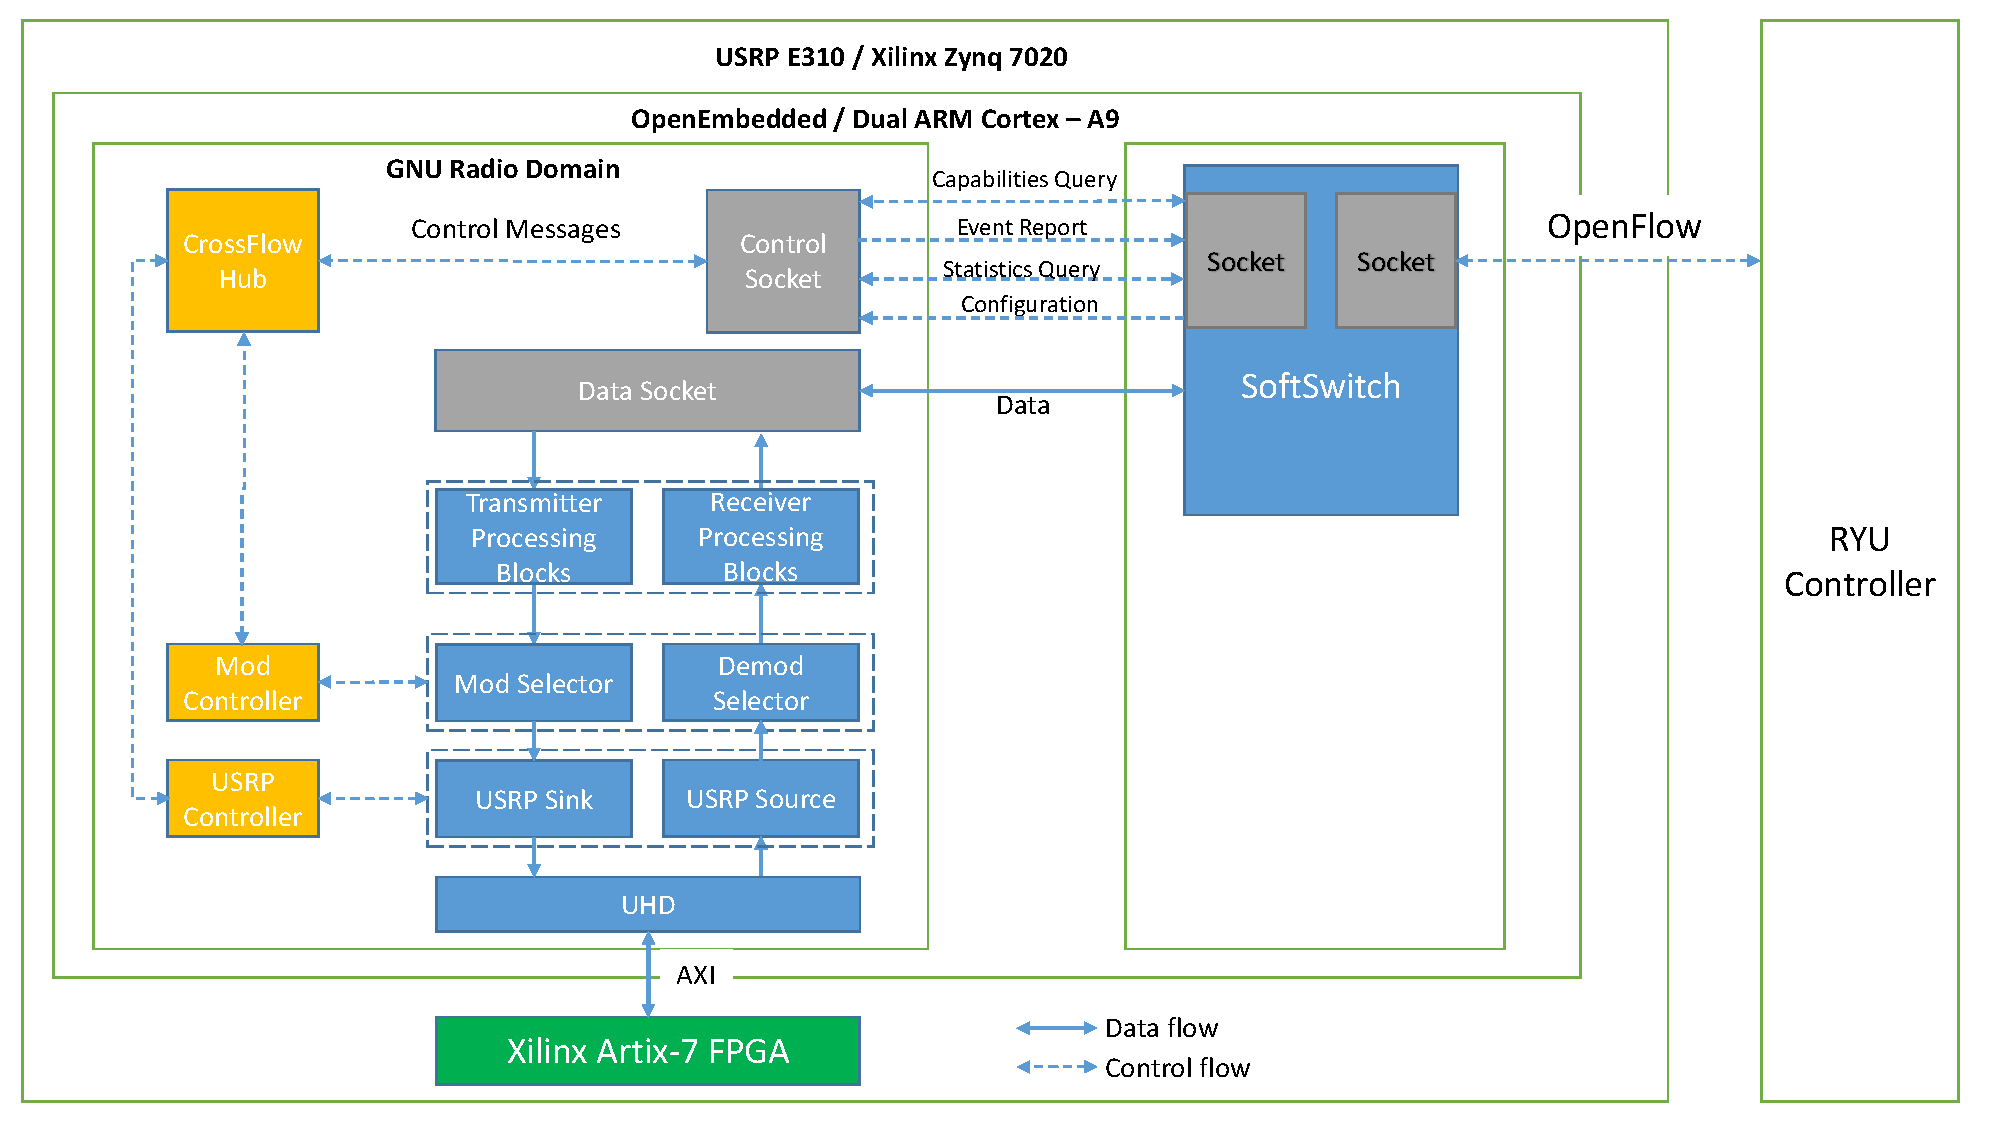
\includegraphics[width=0.8\textwidth]{figures/new.pdf}
%  \caption{Implementation of \crossflow}
%  \label{fig:message_block}
%\end{figure*}

\subsection{Data Plane abstractions}
\label{sec:data_plane}
We extend the data model proposed in \cite{Casey:14} to create an abstraction model for the \crossflow framework, which is displayed in Figure~\ref{fig:uml}. We build upon the \emph{radio physical port} concept proposed in \cite{aetherflow} to create a new layer of abstractions, which we refer to as the \emph{wireless radio port} in this paper. This layer of abstractions exhibits a composition or \emph{has-a} relationship with the \emph{wireless radio port} abstraction (i.e., ``the wireless radio port \emph{has a} sink, modulator, or channel coder). This means that the blocks of this layer are the objects or members that comprise the \emph{wireless radio port}. These blocks are derived from the most commonly used processing blocks in GNU Radio~\cite{gnuradio}. This abstract wireless radio port model serves the following design vision:

\begin{itemize}
\item It allows visibility into the signal processing blocks from an application point of view, without going into implementation details.
\item It allows for the development of an event driven framework for radio operation.
\item It allows composition of blocks to implement new functionality, as this decision is handled by the higher \emph{radio physical port} abstraction. The application simply specifies the blocks to be connected for a specific wireless port instance and the internal framework handles the implementation.
\end{itemize}

In this paper, we focus on the first two bullets. Specifically, we develop an abstract interface to enable event-driven dynamic configuration of signal processing blocks at run-time. We assume that the number of blocks is fixed and the blocks can be connected in a consistent manner. From an application point of view, the application creates instances of the requisite blocks. In order to change parameters, the application needs to send \emph{<command,value>} tuple in a message. For query and receive event responses, it registers for events for each block and during an event, appropriate callbacks are invoked.    
One of the main requirements of the \crossflow model is that each abstraction should implement four types of interfaces as proposed in both \cite{Casey:14} and \cite{aetherflow}, namely: capabilities, configuration, statistics and events. Thus far, CrossFlow provides the interfaces for a wireless radio port abstraction with two processing blocks: \emph{Sink} and \emph{Modulators}. However, we plan to extend it to include the other processing blocks shown in Figure~\ref{fig:uml}. The Sink abstraction allows the SDN controller to manage the signal sinks which can be a USRP device, file or a socket, while the Modulators abstraction allows management of modulation schemes (e.g., BPSK, QPSK, and 8PSK).

The interfaces for \emph{Sink} and \emph{Modulators} are categorized as follows:

%\textbf{Capabilities.}
\textbf{Sink.}
\begin{itemize}
\item \textbf{Capabilities}: The interface allows the SDN controller to query the capabilities of sinks such as:
    (i)  Type of sink (USRP, socket, etc.);
    (ii) Channels supported; 
    (iii) Center Frequency; and
    (iv) IP address. 
\item \textbf{Configuration}: The interface allows the SDN controller to configure properties of signal sinks such as:
    (i) Gain;
    (ii) Frequency, and
    (iii) Sample rate.
\item \textbf{Statistics}: The interface allows the SDN controller to gather statistics for sinks such as:
    (i) Received Signal Strength Indicator (RSSI) and 
    (ii) Temperature on-board.
\item \textbf{Events}: The interface allows the SDN controller to take decisions based upon events in a sink such as:
    (i) Low or high RSSI and
    (ii) Low or high on-board temperature.
\end{itemize}

\textbf{Modulators.}
\begin{itemize}
\item \textbf{Capabilities}: The interface allows the SDN controller to query the properties of the modulator block such as:
    (i) Modulations supported;
    (ii) Current samples/symbol; and 
    (iii) Use of a Gray code indicator.
\item \textbf{Configuration}: The interface allows the SDN controller to configure properties of the modulator block such as:
    (i) Choice of modulation scheme (e.g. BPSK, QPSK and 8PSK); 
    (ii) Sample/symbol; and
    (ii) Use of a Gray code.
\item \textbf{Statistics}: The interface allows the SDN controller to gather statistics for the modulator block such as:
    (i) Signal to Noise Ratio (SNR) and 
    (ii) Bit Error Rate (BER).
\item \textbf{Events}: The interface allows the SDN controller to take decisions based upon events in the modulator block such as:
    (i) Low or high SNR and
    (ii) Low or high BER.
\end{itemize}

\subsection{Message Extensions}
\label{sec:messages}
  		  
\crossflow uses SDN design principles to control a network of configurable SDRs. As such, to enable control plane interactions between the SDN controller and the SDR, we had two options: either we could have implemented our own control protocol to enable their interactions or extend the existing OpenFlow \cite{openflow} framework. This is because OpenFlow does not natively support wireless features. In order to enable a cleaner implementation, we decided to extend OpenFlow by using experimenter messages within the OpenFlow protocol, similar to \aetherflow. Experimenter messages are a part of the standard OpenFlow protocol which provides a mechanism for vendors to include propriety information within the protcol. This provides us with two advantages:
\begin{itemize}
\item We do not need to implement a new protocol for control and data plane interactions.
\item As we are using experimenter messages to carry \crossflow messages, the SDN controller does not need to perform special handling for these messages. This enables the controller to remain independent of the underlying devices and hence it can handle both wired and wireless devices. 
\end{itemize} 
In the current version, we define three messages in \crossflow:
\begin{itemize}
\item Configuration message request - Request for modification of parameters like gain, frequency, SNR threshold and modulation scheme.
\item Statistics message request - Request for statistics such as SNR, BER and RSSI.
\item Event message response - Response for events like SNR below threshold and low BER.
\end {itemize}
